\section{Phá vỡ chưng cất phòng thủ}
Ngoài ra, để tấn công DNN bằng các mẫu đối nghịch, nhóm tác giả đã cho thấy EAD có thể phá vỡ DNN phòng thủ được chưng cất. Phòng thủ distillation (Papernot et al. 2016b) là công nghệ phòng thủ chuẩn mà huấn luyện lại mạng với các xác xuất nhãn từng lớp được dự đoán bởi mạng gốc, nhãn mềm và tham số nhiệt T trong lớp softmax để tăng cường sức mạnh của nó chống lại nhiễu đối nghịch. Tương tự như phương thức tấn công tiên tiến C\&W, hình \ref{fig:fg_03} cho thấy EAD có thể thu được ASR $100\%$ với các giá trị $T$ khác nhau trên tập MNIST và CIFAR10. Hơn nữa, vì công thức tấn công C\&W là trường hợp đặc biệt của công thức EAD trong (\ref{eq:7}) khi $\beta = 0$, sự thành công trong việc phá vỡ phòng thủ chưng cất sử dụng EAD gợi ý 1 cách mới trong việc tạo ra các mẫu đối nghịch hiệu quả bằng cách dùng các tham số  $\beta$ khác nhau cho hiệu chỉnh $L_1$. Kết quả đầy đủ của tấn công ở trong tài liệu mở rộng.

\begin{figure}[H] % places figure environment here   
    \centering % Centers Graphic
    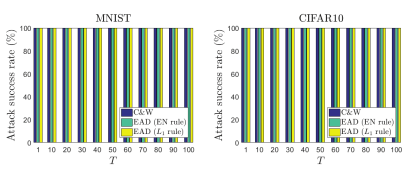
\includegraphics[width=0.8\textwidth]{assets/fig_3.png} 
    \caption{ASR của C\&W và EAD trên tập MNIST và CIFAR10 với các tham số nhiệt T khác nhau cho phòng thủ distill. Cả 2 phương pháp đều phá vỡ thành công phòng thủ distill.} % Creates caption  % Creates caption underneath graph
    \label{fig:fg_03}
\end{figure}